% =====================================================================
%  Betriebsanweisung Oberfräse Festool OF 1010 EBQ
%  Eigenes PDF: Betriebsanweisung_Oberfraese.tex, Seite in der Einweisung
%  über \BAseite. Layout: fablab-document/fablab-ba.sty
%
%  Lizenz-Hinweis: Text vollständig selbst formuliert, KEINE Passagen und
%  KEINE Abbildungen aus der Festool-Betriebsanleitung übernehmen! Sicherheits-
%  regeln als solche (Fakten) sind frei, der Wortlaut und die Bilder von
%  Festool sind urheberrechtlich geschützt. Nur ISO-7010-Symbole und eigene
%  Zeichnungen verwenden.
% =====================================================================
\BAsetup{
  typ=maschine,
  titel={Oberfräse Festool OF 1010 EBQ},
  kurztitel={Oberfräse},
  taetigkeit={Fräsen von Kanten, Nuten und Ausschnitten, Fräserwechsel, Reinigen},
  nummer=BA-OF-01,
  stand=01.10.2026,                   % Datum der Freigabe
  verantwortlich={Name der verantwortlichen Person},
  bildcode={% =====================================================================
%  Kleines Symbol der Oberfräse für den Kopf der Betriebsanweisung
%  (\BAsetup{bildcode=...}). Ohne zeichnungen/stil.tex lauffähig.
%  Selbst gezeichnet.
% =====================================================================
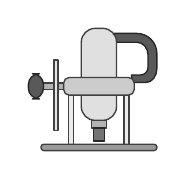
\begin{tikzpicture}[x=0.16mm, y=0.16mm, line width=0.5pt, line join=round]
  % Führungssäulen und Stiel des Drehknopfs
  \draw[fill=black!8, draw=black!75] (-24,5) rectangle (-20,50) (20,5) rectangle (24,50);
  \draw[fill=black!30, draw=black!75] (-44,48.5) rectangle (-28,53.5);
  % Drehknopf und Handgriff
  \draw[fill=black!65, draw=black!85, rounded corners=4] (-56,41) rectangle (-44,61);
  \draw[fill=black!65, draw=black!85] (12,93) -- (30,93) to[out=0,in=90] (46,77) -- (46,65)
    to[out=-90,in=0] (37,54) -- (26,54) -- (26,60) -- (33,60)
    to[out=0,in=-90] (39,66) -- (39,76) to[out=90,in=0] (30,86) -- (12,86) -- cycle;
  % Motor, Spannmutter, Fräser
  \draw[fill=black!12, draw=black!75, rounded corners=5] (-14,24) rectangle (14,97);
  \draw[fill=black!30, draw=black!75] (-6,18) rectangle (6,24);
  \draw[fill=black!55, draw=black!85] (-4.5,7.5) rectangle (4.5,18);
  % Motorträger, Tiefenanschlag, Frästisch
  \draw[fill=black!20, draw=black!75, rounded corners=2] (-28,44) rectangle (28,58);
  \draw[fill=black!10, draw=black!75] (-35.5,16) rectangle (-32.5,72);
  \draw[fill=black!40, draw=black!75, rounded corners=1] (-46,0) rectangle (46,5);
\end{tikzpicture}
},
  schrift=\footnotesize,
}

\BAkopf

\BAblock{ANWENDUNGSBEREICH}{M002}{%
  \begin{itemize}
    \item Fräsen von Holz, Holzwerkstoffen und Kunststoff; Aluminium nur mit geeignetem Fräser.
    \item Handgeführt, mit beiden Händen; Werkstück immer festgespannt.
    \item Benutzung nur nach unterschriebener Einweisung; Betriebsanleitung des Herstellers beachten.
  \end{itemize}}

\BAblock{GEFAHREN FÜR MENSCH UND UMWELT}{W022,W024,W012}{%
  \begin{itemize}
    \item Schnittverletzungen am Fräser, der mit bis zu 24.000 Umdrehungen pro Minute läuft und nach dem Ausschalten noch nachläuft.
    \item \textbf{Gleichlauf:} Fräst man in die falsche Richtung, zieht sich die Fräse selbst ins Material und kann wegspringen.
    \item Wegfliegende Späne oder Fräserbruchstücke; Einzug von Haaren, Schmuck und loser Kleidung; Stromschlag bei angefrästem Netzkabel; Lärm.
    \item Gesundheitsschäden durch Staub; Hartholzstaub kann Krebs erzeugen. Heiße Späne bei Aluminium.
  \end{itemize}}

\BAblock{SCHUTZMASSNAHMEN UND VERHALTENSREGELN}{M003,M004,M017,P028}{%
  \begin{itemize}
    \item Vor jeder Benutzung Fräse, Kabel und Fräser prüfen; nur scharfe, unbeschädigte Fräser verwenden, zulässige Drehzahl des Fräsers beachten.
    \item Gehörschutz tragen; Schutzbrille bei Aluminium, Faserwerkstoffen und Gipskarton; Staubmaske bei viel Staub (Hartholz). Anliegende Kleidung, Haare zusammenbinden. \textbf{Beim Fräsen keine Handschuhe} (Einzugsgefahr); Schutzhandschuhe nur beim Fräserwechsel mit gezogenem Stecker.
    \item Fräser nur bei \textbf{gezogenem Netzstecker} wechseln; Schaft mindestens bis zur Markierung einstecken und fest anziehen.
    \item Werkstück fest spannen, nie mit der Hand halten. Immer Absaugung anschließen (Festool-Sauger, Stellung AUTO).
    \item Fräse mit \textbf{beiden Händen} an den Griffen führen. Erst einschalten, dann eintauchen bzw.\ ans Werkstück führen.
    \item Immer im \textbf{Gegenlauf} fräsen: Außenkanten gegen den Uhrzeigersinn, Ausschnitte im Uhrzeigersinn.
    \item Nach dem Ausschalten warten, bis der Fräser steht, erst dann absetzen. Kabel aus dem Arbeitsbereich fernhalten.
  \end{itemize}}

\BAblock{VERHALTEN BEI STÖRUNGEN UND IM GEFAHRENFALL}{W001,M006}{%
  \begin{itemize}
    \item Fräse ausschalten, Stecker ziehen, Betreuer informieren; Schaden und Hergang per Mail an \texttt{fablab-aktive@fablab.fau.de} melden.
    \item Entstehungsbrand: Fräse vom Netz trennen, löschen. \textbf{Feuerwehr: 112}
  \end{itemize}}

\BAblock{VERHALTEN BEI UNFÄLLEN – ERSTE HILFE}{E003}{%
  \begin{itemize}
    \item Fräse ausschalten, Stecker ziehen. Betreuer/Ersthelfer verständigen, Wunden versorgen.
    \item Jeden Unfall melden und im Verbandbuch eintragen.
  \end{itemize}\vspace{1.5mm}
  \textbf{Notruf: 112}\qquad FabLab: 09131\,/\,85\,28013}

\BAletzterblock{INSTANDHALTUNG, ENTSORGUNG}{M021}{%
  \begin{itemize}
    \item Wartung nur durch eingewiesene Personen mit gezogenem Stecker.
    \item Fräse nach jeder Benutzung aussaugen; Druckluft nur im Freien bzw.\ aus dem Fenster. Elektrische Prüfung nach DGUV Vorschrift 3 gemäß Prüffrist.
  \end{itemize}}
